\section{Resultados y Análisis}
En esta sección presentaremos y analizaremos los resultados obtenidos al correr los distintos test propuestos.
Para ello correremos los mismos con una iteración de 100 repeticiones sobre los host de las siguientes universidades.

\subsection{Universidad de Tokyo}
El host de destino de la universidad de Tokyo sera el dominio ``www.u-tokyo.ac.jp'' cuya IP es ``210.152.135.178''. El host de la universidad de Tokyo se encuentra ubicado la ciudad de Tokyo, Japón. El origen sera un host ubicado en la Ciudad de Buenos Aires, Argentina utilizando como isp a Telecentro.

\subsubsection{Datos}

Los datos obtenidos para este caso fueron los siguientes:

\begin{table}[H]
    \begin{center}
        \begin{tabular}{| r | r | r | r | r |}
  \hline
  {\bf TTL} & \multicolumn{1}{|c|}{\bf IP} & {\bf E(RTT) (ms)} & {\bf S(RTT) (ms)} & {\bf $\Delta$RTT (ms)}\\
  \hline
\hline 1  & 192.168.10.1 & 0.414 & 0.025 & 0.414\\
\hline 2  & 10.20.64.1 & 9.588 & 2.179 & 9.174\\
\hline 3  & 200.115.194.173 & 9.709 & 2.050 & 0.121\\
\hline 4  & 208.178.195.210 & 11.823 & 2.660 & 2.114\\
\hline 5  & 208.178.195.209 & 10.154 & 3.919 & 0.000\\
\rowcolor{blue!25}\hline 6  & 64.212.107.98 & 140.102 & 2.736 & 129.948\\
\hline 7  & 129.250.3.172 & 141.972 & 6.459 & 1.870\\
\hline 8  & 129.250.2.219 & 165.020 & 5.163 & 23.048\\
\hline 9  & 129.250.7.69 & 174.848 & 10.839 & 9.828\\
\rowcolor{blue!25}\hline 10  & 129.250.2.177 & 289.040 & 10.215 & 114.191\\
\hline 11  & 129.250.6.144 & 286.955 & 9.046 & 0.000\\
\hline 12  & 61.200.80.218 & 281.767 & 6.327 & 0.000\\
\hline 13  & 158.205.192.173 & 287.145 & 8.005 & 5.378\\
\hline 14  & 158.205.192.86 & 300.318 & 5.018 & 13.173\\
\hline 15  & 158.205.121.250 & 299.293 & 22.325 & 0.000\\
\hline 16  & 154.34.240.254 & 287.327 & 2.431 & 0.000\\
\hline 17  & 210.152.135.178 & 300.554 & 3.888 & 13.227\\
\hline
        \end{tabular}
        \caption{$\overline{RTT}$, $\sigma$RTT y $\Delta$RTT para la ruta utilizada para llegar www.u-tokyo.ac.jp}
        \label{table:tokyo} 
    \end{center}
\end{table}

Analizando la información aportada por la tabla \ref{table:tokyo} podemos notar que tanto el salto 6 como 10 sobresalen por sobre el resto en cuanto a sus tiempos de $\Delta$RTT. 

\subsubsection{RTT y $\Delta$RTT}

\begin{figure}[H]
    \begin{center}
        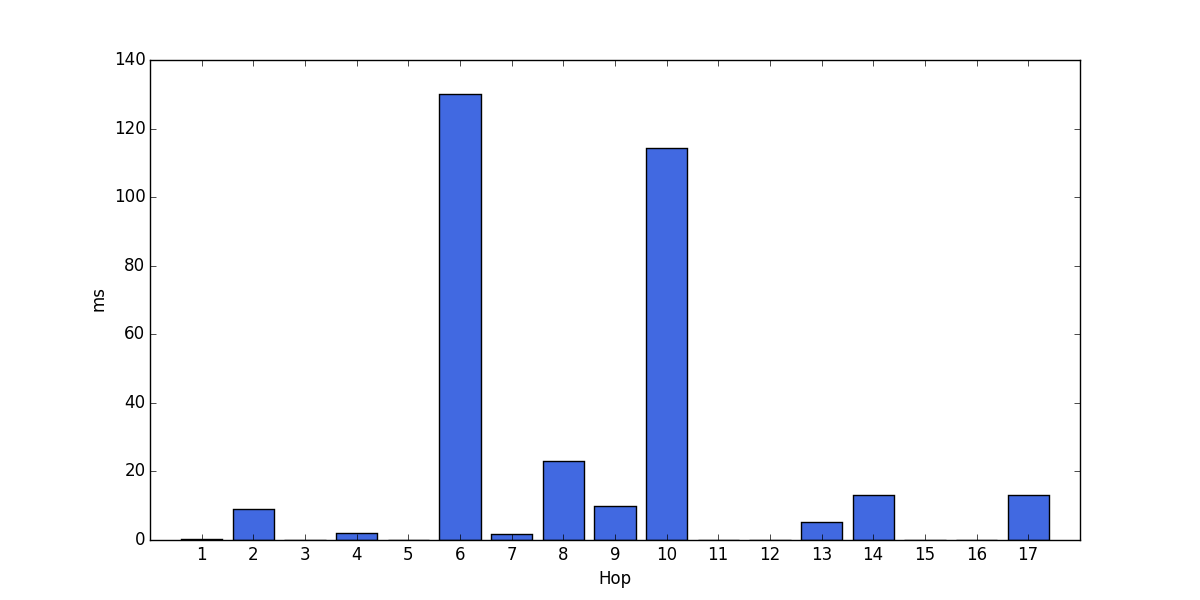
\includegraphics[width=1\textwidth]{data/rtt-tokyo-bar.png}
        \caption{www.u-tokyo.ac.jp - $\Delta$RTT}
        \label{histo:tokyo}
    \end{center}
\end{figure}

\begin{figure}[H]
    \begin{center}
        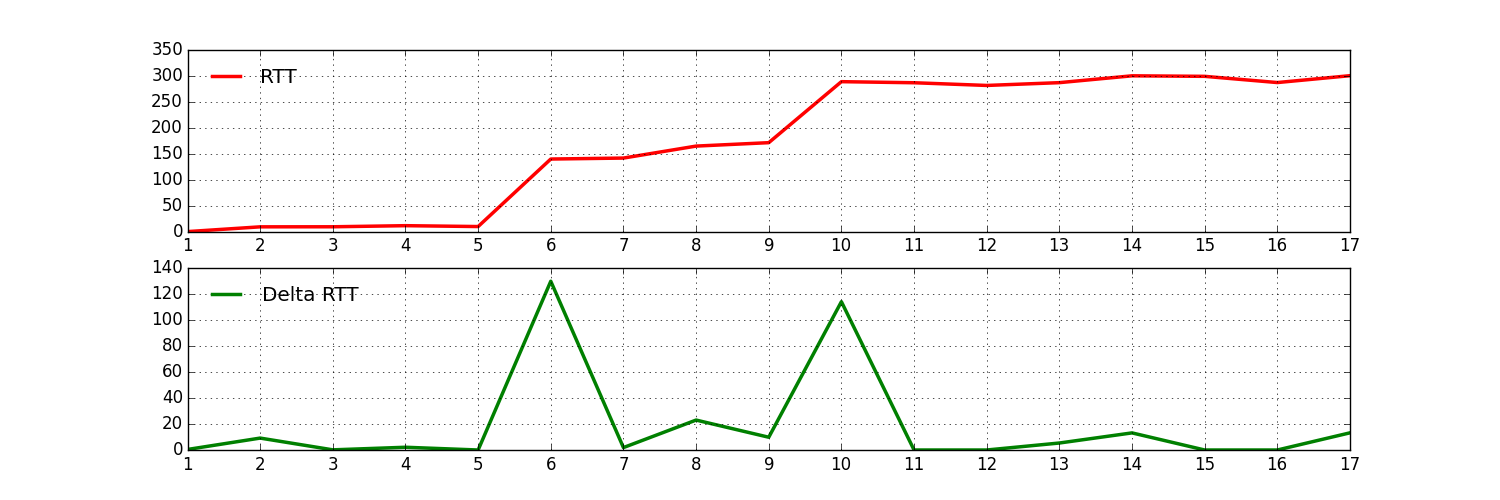
\includegraphics[width=1\textwidth]{data/rtt-tokyo-lines.png}
        \caption{www.u-tokyo.ac.jp - RTT y $\Delta$RTT}
        \label{lines:tokyo}
    \end{center}
\end{figure}

Tanto en la figura \ref{histo:tokyo} como en la figura \ref{lines:tokyo} podemos comprobar los que habíamos notado en la tabla \ref{table:tokyo}. Esto es que tanto el salto 6 como 10 se destacan por sobre el resto. En caso de existir algún enlace submarino seguramente este se correspondería con alguno de estos saltos. Esto lo analizaremos en las siguientes secciones.

\subsubsection{Test de Grubbs}\label{tokyo:grubbs}

\subsubsection{Geolocalización}

\begin{table}[H]
    \begin{center}
        \begin{tabular}{| r | r | c | c |}
  \hline
  {\bf TTL} & \multicolumn{1}{|c|}{\bf IP} & {\bf DNS} & {\bf Ubicación}\\
  \hline
\hline 1  & 192.168.10.1 & rig0.tuxhome.com.ar(ip privada) &\\
\hline 2  & 10.20.64.1 & no disponible(ip privada) &\\
\hline 3  & 200.115.194.173 & cpe-200-115-194-173.telecentro-reversos.com.ar & Buenos Aires, Argentina\\
\hline 4  & 208.178.195.210 & global-crossing-argentina-s-a.xe-0-1-0.ar3... & Buenos Aires, Argentina \\
\hline 5  & 208.178.195.209 & xe-0-1-0.ar3.eze1.gblx.net & Buenos Aires, Argentina \\
\rowcolor{blue!25}\hline 6  & 64.212.107.98 & no disponible  & Los Angeles, Usa\\
\hline 7  & 129.250.3.172 & ae-4.r21.miamfl02.us.bb.gin.ntt.net & Miami, Usa \\
\hline 8  & 129.250.2.219 & ae-4.r22.dllstx09.us.bb.gin.ntt.net & Dallas, Usa\\
\hline 9  & 129.250.7.69 & ae-5.r22.lsanca07.us.bb.gin.ntt.net & Los Angeles, Usa\\
\rowcolor{blue!25}\hline 10  & 129.250.2.177 & ae-0.r21.osakjp02.jp.bb.gin.ntt.net & Houston, Usa\\
\hline 11  & 129.250.6.144 & ae-5.r23.osakjp02.jp.bb.gin.ntt.net & Osaka, Japan\\
\hline 12  & 61.200.80.218 & xe-1-1-10.r23.osakjp02.jp.ce.gin.ntt.net & Osaka, Japan\\
\hline 13  & 158.205.192.173 & ae0.ostcr01.idc.jp & Tokyo, Japan\\
\hline 14  & 158.205.192.86 & no disponible  & Tokyo, Japan\\
\hline 15  & 158.205.121.250 & po2.l321.fk1.eg.idc.jp & Tokyo, Japan\\
\hline 16  & 154.34.240.254 & no disponible & Tokyo, Japan\\
\hline 17  & 210.152.135.178 & www.u-tokyo.ac.jp & Tokyo, Japan\\
\hline
        \end{tabular}
        \caption{Ruta utilizada para llegar www.u-tokyo.ac.jp con la ubicación de los diferentes saltos por los que se pasa. Se encuentran resaltados los saltos distinguidos calculados en la sección \ref{tokyo:grubbs}}
        \label{table:tokyo} 
    \end{center}
\end{table}

En la tabla \ref{table:tokyo} notamos que el salto 10 figura ubicado en Houston, Estados Unidos, sin embargo dado el $\Delta$RTT de este salto que hizo que sea distinguido como outlier en la la sección \ref{tokyo:grubbs} y su DNS reverso ``ae-0.r21.osakjp02.jp.bb.gin.ntt.net'' inferimos que es un error en las bases de datos de geolocalización y que ese salto se encuentra efectivamente ubicado en Osaka, Japon. Por este motivo al trazar el traceroute sobre el mapa de la figura \ref{mapa:tokyo} lo ubicamos en esta última localidad.

\begin{figure}[H]
    \begin{center}
        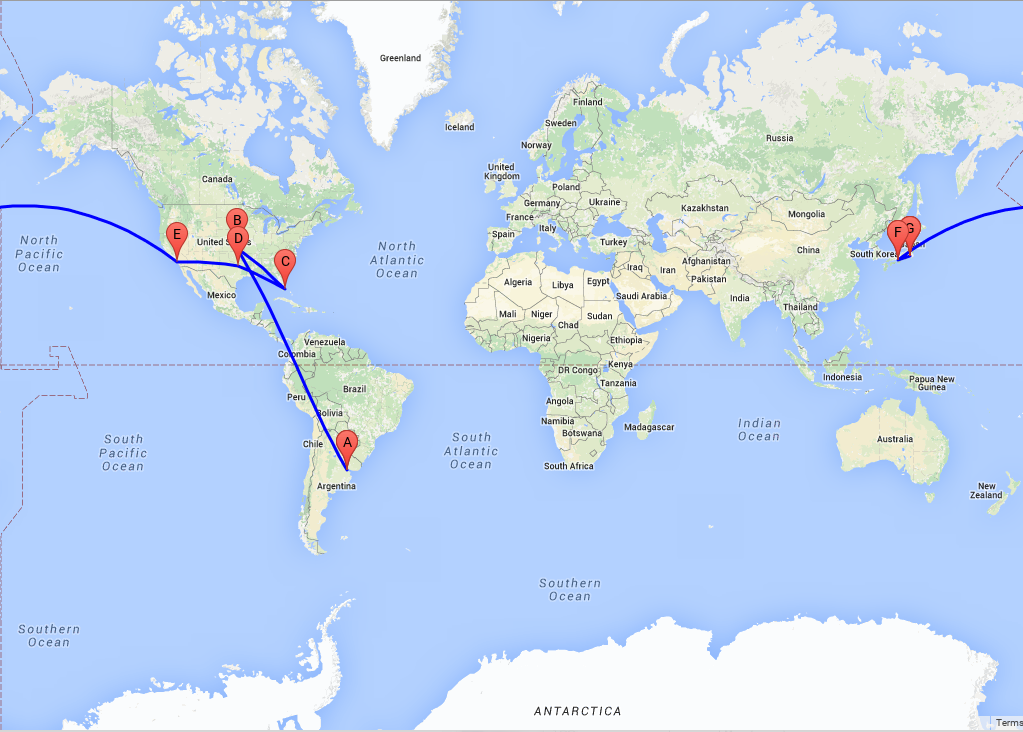
\includegraphics[width=1\textwidth]{data/mapa-tokyo.png}
        \caption{www.u-tokyo.ac.jp - Traceroute}
        \label{mapa:tokyo}
    \end{center}
\end{figure}

\subsection{Universidad de Pretoria}
El host de destino de la universidad de Pretoria sera el dominio ``www.up.ac.za'' cuya IP es ``5.10.110.85''. El host de la universidad de Pretoria se encuentra ubicado la ciudad de Pretoria, en sudáfrica. El origen es un host ubicado en la Ciudad de Buenos Aires, Argentina utilizando como isp a Telecentro.

\subsubsection{Datos}

Los datos obtenidos para este caso fueron los siguientes:

\begin{table}[H]
    \begin{center}
        \begin{tabular}{| r | r | r | r | r |}
  \hline
  {\bf TTL} & \multicolumn{1}{|c|}{\bf IP} & {\bf E(RTT) (ms)} & {\bf S(RTT) (ms)} & {\bf $\Delta$RTT (ms)}\\
  \hline 
\hline 1  & 192.168.0.1 &  3.037 & 3.218 & 3.037\\
\rowcolor{blue!25}\hline 2  & 10.19.0.1 & 21.794 & 23.114 & 18.757\\
\hline 3  & 200.115.195.81 & 19.089 & 14.663 & 0.000\\
\hline 4  & 208.178.195.214 & 20.840 & 13.042 & 1.751\\ 
\hline 5  & 208.178.195.213 & 22.422 & 18.565 & 1.582\\ 
\rowcolor{blue!25}\hline 6  & 67.17.75.66 & 158.745 & 28.768 & 136.323\\ 
\hline 7  & 4.68.111.121 &  152.379 & 26.292 & 0.000\\ 
\rowcolor{blue!25}\hline 8  & 4.69.168.11 & 272.512 & 19.879 & 120.133\\ 
\hline 9  & 4.69.168.11 & 277.326 & 26.226 & 4.814\\ 
\rowcolor{blue!25}\hline 10  & 212.73.206.174 & 292.420 & 28.952 & 15.094\\ 
\hline 11  & 50.97.19.101 & 281.778 & 31.841 & 0.000\\ 
\hline 12  & 50.97.19.41 & 289.224 & 33.909 & 7.446\\ 
\hline 13  & 5.10.118.135 & 278.807 & 23.145 & 0.000\\ 
\hline 14  & 5.10.110.85 & 279.282 & 18.527 & 0.476\\ 
\hline
        \end{tabular}
        \caption{$\overline{RTT}$, $\sigma$RTT y $\Delta$RTT para la ruta utilizada para llegar www.up.ac.za}
        \label{table:pretoria} 
    \end{center}
\end{table}

Analizando la información aportada por la tabla \ref{table:pretoria} podemos notar que los saltos 2, 6, 8 y 10 sobresalen por sobre el resto en cuanto a sus tiempos de $\Delta$RTT. 

\subsubsection{RTT y $\Delta$RTT}

\begin{figure}[H]
    \begin{center}
        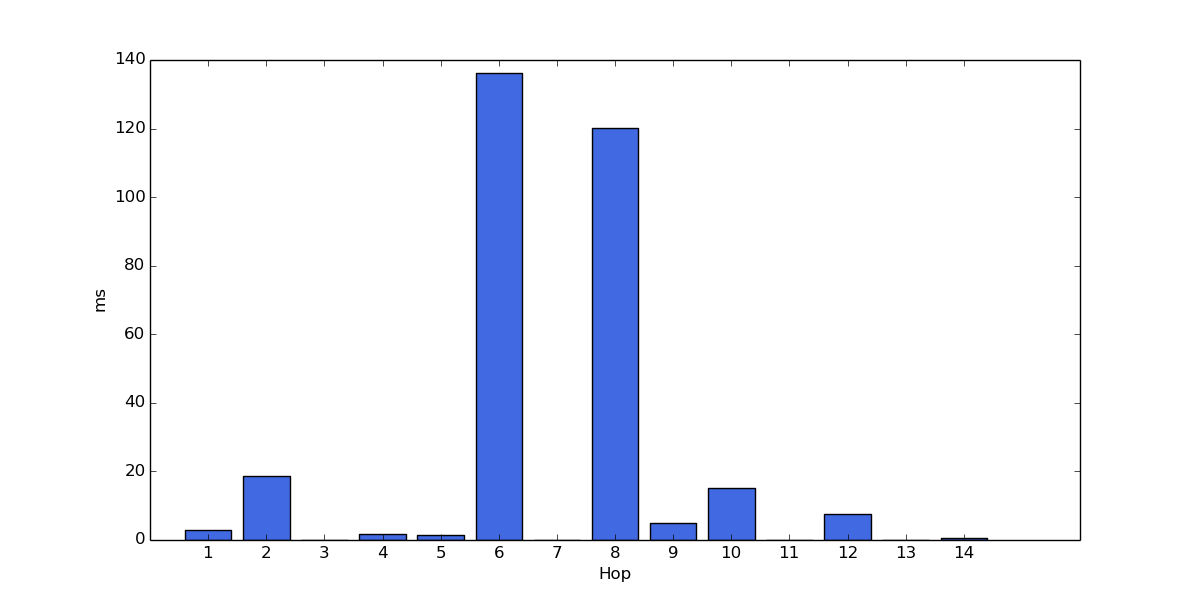
\includegraphics[width=1\textwidth]{data/rtt-pretoria-bar.png}
        \caption{www.up.ac.za - $\Delta$RTT}
        \label{histo:pretoria}
    \end{center}
\end{figure}

\begin{figure}[H]
    \begin{center}
        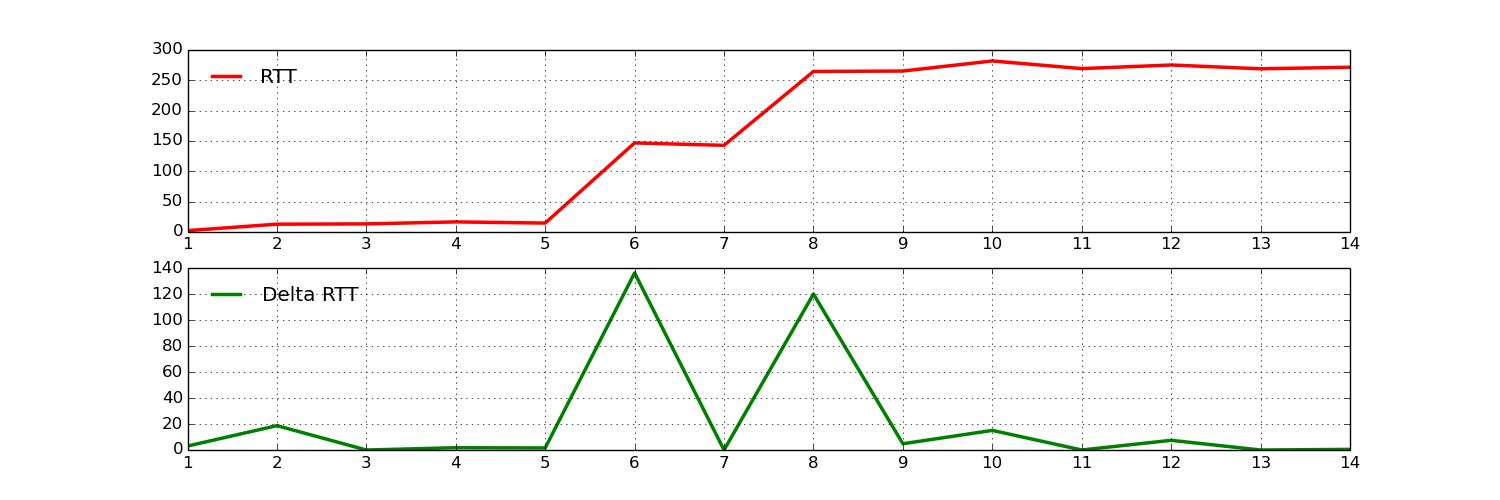
\includegraphics[width=1\textwidth]{data/rtt-pretoria-lines.png}
        \caption{www.up.ac.za - RTT y $\Delta$RTT}
        \label{lines:pretoria}
    \end{center}
\end{figure}

Tanto en la figura \ref{histo:pretoria} como en la figura \ref{lines:pretoria} podemos comprobar los que habíamos notado en la tabla \ref{table:pretoria}. Esto es que tanto los saltos 2, 6, 8 y 10 se destacan por sobre el resto. En caso de existir algún enlace submarino seguramente este se correspondería con alguno de estos saltos. Esto lo analizaremos en las siguientes secciones.

\subsubsection{Test de Grubbs}\label{pretoria:grubbs}

\subsubsection{Geolocalización}

\begin{table}[H]
    \begin{center}
        \begin{tabular}{| r | r | c | c |}
  \hline
  {\bf TTL} & \multicolumn{1}{|c|}{\bf IP} & {\bf DNS} & {\bf Ubicación}\\
  \hline
\hline 1  & 192.168.0.1 & (ip privada) & \\
\rowcolor{blue!25}\hline 2  & 10.19.0.1 & (ip privada) & \\
\hline 3  & 200.115.195.81 & cpe-200-115-195-81.telecentro-reversos.com.ar & Buenos Aires, Argentina\\
\hline 4  & 208.178.195.214 & global-crossing-argentina-s-a.xe-0-3-1.ar3.eze1.gblx.net & Virginia, USA\\ 
\hline 5  & 208.178.195.213 & xe-0-3-1.ar3.eze1.gblx.net & Virginia, USA\\ 
\rowcolor{blue!25}\hline 6  & 67.17.75.66 &  po3-20G.ar3.MIA2.gblx.net & Miami, USA\\ 
\hline 7  & 4.68.111.121 &  ae5.edge2.miami2.level3.net  & Miami, USA\\ 
\rowcolor{blue!25}\hline 8  & 4.69.168.11 & ae-1-60.ear1.Paris1.Level3.net & Paris, Francia\\ 
\hline 9  & 4.69.168.11 & ae-1-60.ear1.Paris1.Level3.net & Paris, Francia\\ 
\rowcolor{blue!25}\hline 10  & 212.73.206.174 & unknown.Level3.net & Los Angeles, USA\\ 
\hline 11  & 50.97.19.101 & ae1.bbr02.tg01.lon01.networklayer.com & Londres, Inglaterra\\ 
\hline 12  & 50.97.19.41 & ae6.dar01.lon02.networklayer.com & Londres, Inglaterra\\ 
\hline 13  & 5.10.118.135 & po1.fcr01b.lon02.networklayer.com & Londres, Inglaterra\\ 
\hline 14  & 5.10.110.85 &  55.6e.0a05.ip4.static.sl-reverse.com & Londres, Inglaterra\\ 
\hline
        \end{tabular}
        \caption{Ruta utilizada para llegar www.up.ac.za con la ubicación de los diferentes saltos por los que se pasa. Se encuentran resaltados los saltos distiguidos calculados en la seccion \ref{pretoria:grubbs}}
        \label{table:pretoria} 
    \end{center}
\end{table}
>>>>>>> 4e2bf230d534ad9b6017fbb58a1c9aee477a8153
